\chapter{微分几何与张量分析}
这一章节从两个角度来写.第一是形象的微分几何,比如曲线理论、曲面理论.第二是抽象的微分几何,比如流形理论.

\section{曲线理论}
\subsection{曲线的表示}
曲线有平面与空间曲线,后者一般可以从前者扩展面来.

\subsubsection{参数表示法}
\begin{empheq}[left=\empheqlbrace]{align*}
x&=x(t)\\
y&=y(t)
\end{empheq}
也可以用向量来表示
$$\bm{r}=\bm{r}(t)$$

\subsubsection{隐式表示}
用方程表示
$$F(x,y)=0$$

\subsubsection{弧长表示}
将曲线坐标表示为弧长的函数
$$\bm{r}=\bm{r}(s)$$

这种表示法比较难算,因为弧长是积分.但后面可以看到,弧长表示法易于表达曲率、挠率等概念.

以下用$t$表示一般参数表达,用$s$表示弧长表达.

\subsection{与曲线有关的量}
\subsubsection{弧长}
\begin{empheq}{align*}
s&=\int_{a}^{b} \sqrt{x'(t)^2+y'(t)^2}\dif t \mtag{平面曲线}\\
&=\int_{a}^{b} \sqrt{x'(t)^2+y'(t)^2+z'(t)^2}\dif t \mtag{空间曲线}\\
&=\int_{a}^{b} |\bm{r}'(t)| \dif t
\end{empheq}

\subsubsection{切向量}
就是梯度$\bm{t}=\bm{r}'(s)$.
\subsubsection{曲率}
与二阶导数有关.
\begin{empheq}{align*}
k&=\frac{x'y''-y'x''}{(x'^2+y'^2)^{\frac{3}{2}}} \mtag{平面曲线}\\
&=|\bm{r}''(s)|\\
R&=\frac{1}{|k|} \mtag{曲率半径}
\end{empheq}

\subsubsection{单位法向量}
$$\bm{n}=\frac{1}{k}\bm{r}''(s)$$
\subsubsection{副法向量}
$$\bm{b}=\bm{t}\bm{n}$$
\subsubsection{挠率}
三阶导数.

\subsubsection{奇点}
即导数为0的点,即$\bm{r}'(t)=0$.

\subsection{各种平面曲线}
\subsubsection{椭圆}

\subsection{各种空间曲线}

\section{曲面理论}
\subsection{曲面的表示}
\subsubsection{第一基本型}
给定曲面$\bm{r}(u,v)$,$\bm{r}$是三维向量。则第一基本型的系数为$E,F,G$,则线元素为
$$I=E\dif u^2+2F\dif u\dif v+G\dif v^2$$
其中
\begin{empheq}{align*}
E&=\bm{r}_u\cdot \bm{r}_u\\
F&=\bm{r}_u\cdot \bm{r}_v\\
G&=\bm{r}_v\cdot \bm{r}_v
\end{empheq}
所谓线元素是指线段$\bm{r}(u,v)$到$\bm{r}(u+\dif u,v+\dif v)$的长度。

从形式上看,第一基本型与度量张量\eqref{metric-tensor}的表示一模一样。其实
\begin{empheq}[left=\empheqlbrace]{align*}
E&=g_{11}\\
F&=g_{12}=g_{21}\\
G&=g_{22}
\end{empheq}

可以看出,曲面相当于$R^2\rightarrow R^3$的映射,而一般的坐标变换是$R^n\rightarrow R^n$的映射,在两种情况下都可以计算度规。

面积元为
$$\dif A=|\bm{r}_u\times \bm{r}_v|\dif u\dif v=\sqrt{|g|}\dif u\dif v$$

\subsubsection{第二基本型}
给定曲面$\bm{r}=\bm{r}(u,v)$
$$II = L\dif u^2 + 2M \dif u\dif v+N\dif v^2$$
其中
\begin{empheq}{align*}
\bm{n}&=\frac{\bm{r}_u\times \bm{r}_v}{|\bm{r}_u\times \bm{r}_v|}\\
L&=\bm{r}_{uu}\cdot \bm{n}\\
M&=\bm{r}_{uv}\cdot \bm{n}\\
N&=\bm{r}_{vv}\cdot \bm{n}
\end{empheq}

第二基本型的实质是邻近点到切平面的有向距离。对于一个点$\bm{r}(u_0,v_0)$,该点处法向量为$\bm{n}$,取切平面$\pi$,再取一个邻近点$\bm{r}(u+\Delta u,v+\Delta v)$,则点到$\pi$的有向距离是
$$\delta(\Delta u,\Delta v)=(\bm{r}(u+\Delta u,v+\Delta v)-\bm{r}(u,v))\cdot\bm{n}=\frac{1}{2}II+o(\Delta^2 u+\Delta^2 v)$$

显然,第二基本型可以用来表示曲面的弯曲程度,某点处的值越大,表示微扰带来的偏离越远,则弯曲得越厉害。

\subsubsection{作为曲面的3D函数}
考虑一个3D函数$f(x,y)$,取曲面$\bm{r}(u,v,f(u,v))$。则
\begin{empheq}{align*}
\bm{r}_u&=(1,0,f_u)\\
\bm{r}_v&=(0,1,f_v)\\
\bm{n}&=\frac{(-f_u,-f_v,1)}{\sqrt{f_u^2+f_v^2+1}}\\
\bm{r}_{uu}&=(0,0,f_{uu})\\
\bm{r}_{uv}&=(0,0,f_{uv})\\
\bm{r}_{vv}&=(0,0,f_{vv})\\
J&=\begin{bmatrix}
\bm{r}_u&\bm{r}_v
\end{bmatrix}\\
G_{ij}&=J^TJ=\begin{bmatrix}
1+(f_u)^2&f_uf_v\\
f_vf_u&1+(f_v)^2
\end{bmatrix}\\
G^{ij}&=G_{ij}^{-1}=\inv{(f_u)^2+(f_v)^2+1}\begin{bmatrix}
1+(f_v)^2&-f_uf_v\\
-f_uf_v&1+(f_u)^2
\end{bmatrix}
\end{empheq}

Christoffel符号有8个:$1\leq i,j,k\leq 2$。
\subsection{曲面的性质}
\subsubsection{测地线}
测地线是测地曲率为0的点,是直线概念的推广,但在任意维的流形上,测地线不一定是最短的,不过最短的一定是测地线。也就是说测地线可能不惟一。

在黎曼度量下,对于三维曲面,其含义是
\begin{empheq}[box=\fbox]{equation}
\frac{D}{\dif  t}\left(\odv{\bm{r}(u(t),v(t))}{t}\right)
\end{empheq}

任意维的度量中,测地线按以下方程组给出:
\begin{empheq}[box=\fbox]{equation}
\pdv[order={2}]{u^i}{t}+\Gamma^i_{jk}\pdv{u^j}{t}\pdv{u^k}{t}=0,1\leq i\leq n
\end{empheq}
注意这里$u,v$实际上是单参数函数。

初始条件可以按两种方式给出,一是边值问题,即给定起点$[u(0),v(0)]$与终点$[u(1),v(1)]$。二是初值问题,给定起点$[u(0),v(0)]$与方向$[u'(0),v'(0)]$。对于三维曲面$f(u,v)$,测地线由参数方程$[u[t],v[t],f(u[t],v[t])]$给出。

但是黎曼度量在代数曲面上可能难以计算,所以还是从测地曲率的角度考虑比较好。

\section{超曲面}
\subsection{超曲面上的几何}
\subsubsection{切丛}
给定一个$n$元函数$F(\bx)$,其在某点$\bm{p}_0$处的梯度为$\nabla F(\bm{p}_0)$,等值面为$F(\bx)=F(\bm{p}_0)$,维度是$n-1$,等值面的法向量为$\nabla F(\bm{p}_0)$(法向量是梯度),$tF(\bm{p}_0)$为法向量空间,其维度是$1$,等值面在该点处的切空间为$\nabla F(\bm{p}_0)\cdot \bx-\nabla F(\bm{p}_0)\cdot\bm{p}_0=0$(切空间过点,且垂直于梯度)。所以说某点等值面的法向量就是函数的梯度。

另一方面,$n$元函数可以视为一个$n+1$维平面$F(\bx)-x_{n+1}=0$,该点处的切空间为
$$\begin{bmatrix}
\nabla F(\bm{p}_0) & -1
\end{bmatrix}\cdot \begin{bmatrix}
\bx & x_{n+1}
\end{bmatrix}=\begin{bmatrix}
\nabla F(\bm{p}_0) & -1
\end{bmatrix}\cdot \begin{bmatrix}
\bm{p}_0 & F(\bm{p}_0)
\end{bmatrix}$$
或者
\begin{empheq}{align*}
x_{n+1}&=\nabla F(\bm{p}_0)\cdot \bx-(\nabla F(\bm{p}_0)\cdot \bm{p}_0-F(\bm{p}_0))\\
&=F(\bm{p}_0)+\nabla F(\bm{p}_0) \cdot ( \bx-\bm{p}_0)
\end{empheq}
注意,这里其实就是一阶泰勒展开,所以切平面相当于一阶泰勒展开式。注意第一项是偏移量,第二项是等值面的切空间。
\subsection{曲面理论定理}
\section{张量与场}
\subsection{度规与联络}\label{tensor-field-metric}
度规(或者度量张量)的含义是:
\begin{empheq}[box=\fbox]{equation}
\dif s^2=g_{ij}\dif x^i \dif x^j\label{metric-tensor}
\end{empheq}

对于曲面坐标系中的张量,有:
\begin{empheq}[box=\fbox]{align}
A_i&=g_{ik}A^k
\end{empheq}

给定坐标系$x_i=x_i(x^i,x^j,x^k)$,$x_i$是欧几里得坐标(一般用下标表示),则
\begin{empheq}{align}
g_{ij}&=\sum_{i=1}^{3}\pdv{x_k}{x^i}\pdv{x_k}{x^j}\\
g^{ij}&=\sum_{i=1}^{3}\pdv{x^i}{x^k}\pdv{x^j}{x^k}
\end{empheq}
注意,$g_{ij}$和$g^{ij}$通常是$x^i$的函数,即曲线坐标。它也可以用矩阵形式表示:
\begin{empheq}{align}
(g_{ij})=J^TJ=G\\
(g^{ij})=G^{-1}
\end{empheq}
$J$为Jacobi矩阵:
\[J=\pdv{{(x_1,x_2,x_3)}}{{(x^1,x^2,x^3)}}=\begin{bmatrix}
\pdv{x_1}{x^1} &\pdv{x_1}{x^2}&\pdv{x_1}{x^3}\\
\pdv{x_2}{x^1} &\pdv{x_2}{x^2}&\pdv{x_2}{x^3}\\
\pdv{x_3}{x^1} &\pdv{x_3}{x^2}&\pdv{x_3}{x^3}
\end{bmatrix}\]


度规的导数与协变导数按下式给出:
\begin{empheq}{align*}
	\pdv{g^{ik}}{x^l}&=-\Gamma^i_{ml}g^{mk}-\Gamma^k_{ml}g^{im}\\
	g^{ik}_{;l}&=g_{ik;l}=0
\end{empheq}

\subsection{Christoffel符号}
\begin{empheq}[box=\fbox]{align}
\Gamma_{i,kl}&=\frac{1}{2}\left(\pdv{g_{ik}}{x^l}+\pdv{g_{il}}{x^k}-\pdv{g_{kl}}{x^i}\right)\\
\Gamma^i_{jk}&=\frac{1}{2}g^{im}\left(\pdv{g_{mk}}{x^l}+\pdv{g_{ml}}{x^k}-\pdv{g_{kl}}{x^m}\right)=g^{im}\Gamma_{m,kl}
\end{empheq}

\subsection{协变导数}
张量的协变导数定义为
\begin{empheq}[box=\fbox]{align}
DA_i&=g_{ik}DA^k\label{DA_ig}\\
	DA^{ik}&=\dif A^{ik}-\delta A^{ik}\equiv A^{ik}_{;l}\dif x^l\mtag{协变微分}\\
A^{ik}_{;l}&=\pdv{A^{ik}}{x^l}+\Gamma^i_{ml}A^{mk}+\Gamma^k_{ml}A^{im}\\
A^i_{k;l}&=\pdv{A^i_k}{x^l}-\Gamma^m_{kl}A^i_m+\Gamma^i_{ml}A^m_k\\
A_{ik;l}&=\pdv{A_{ik}}{x^l}-\Gamma^m_{il}A_{mk}+\Gamma^m_{kl}A_{im}
\end{empheq}

协变微分可以按如下方式理解。
\begin{center}
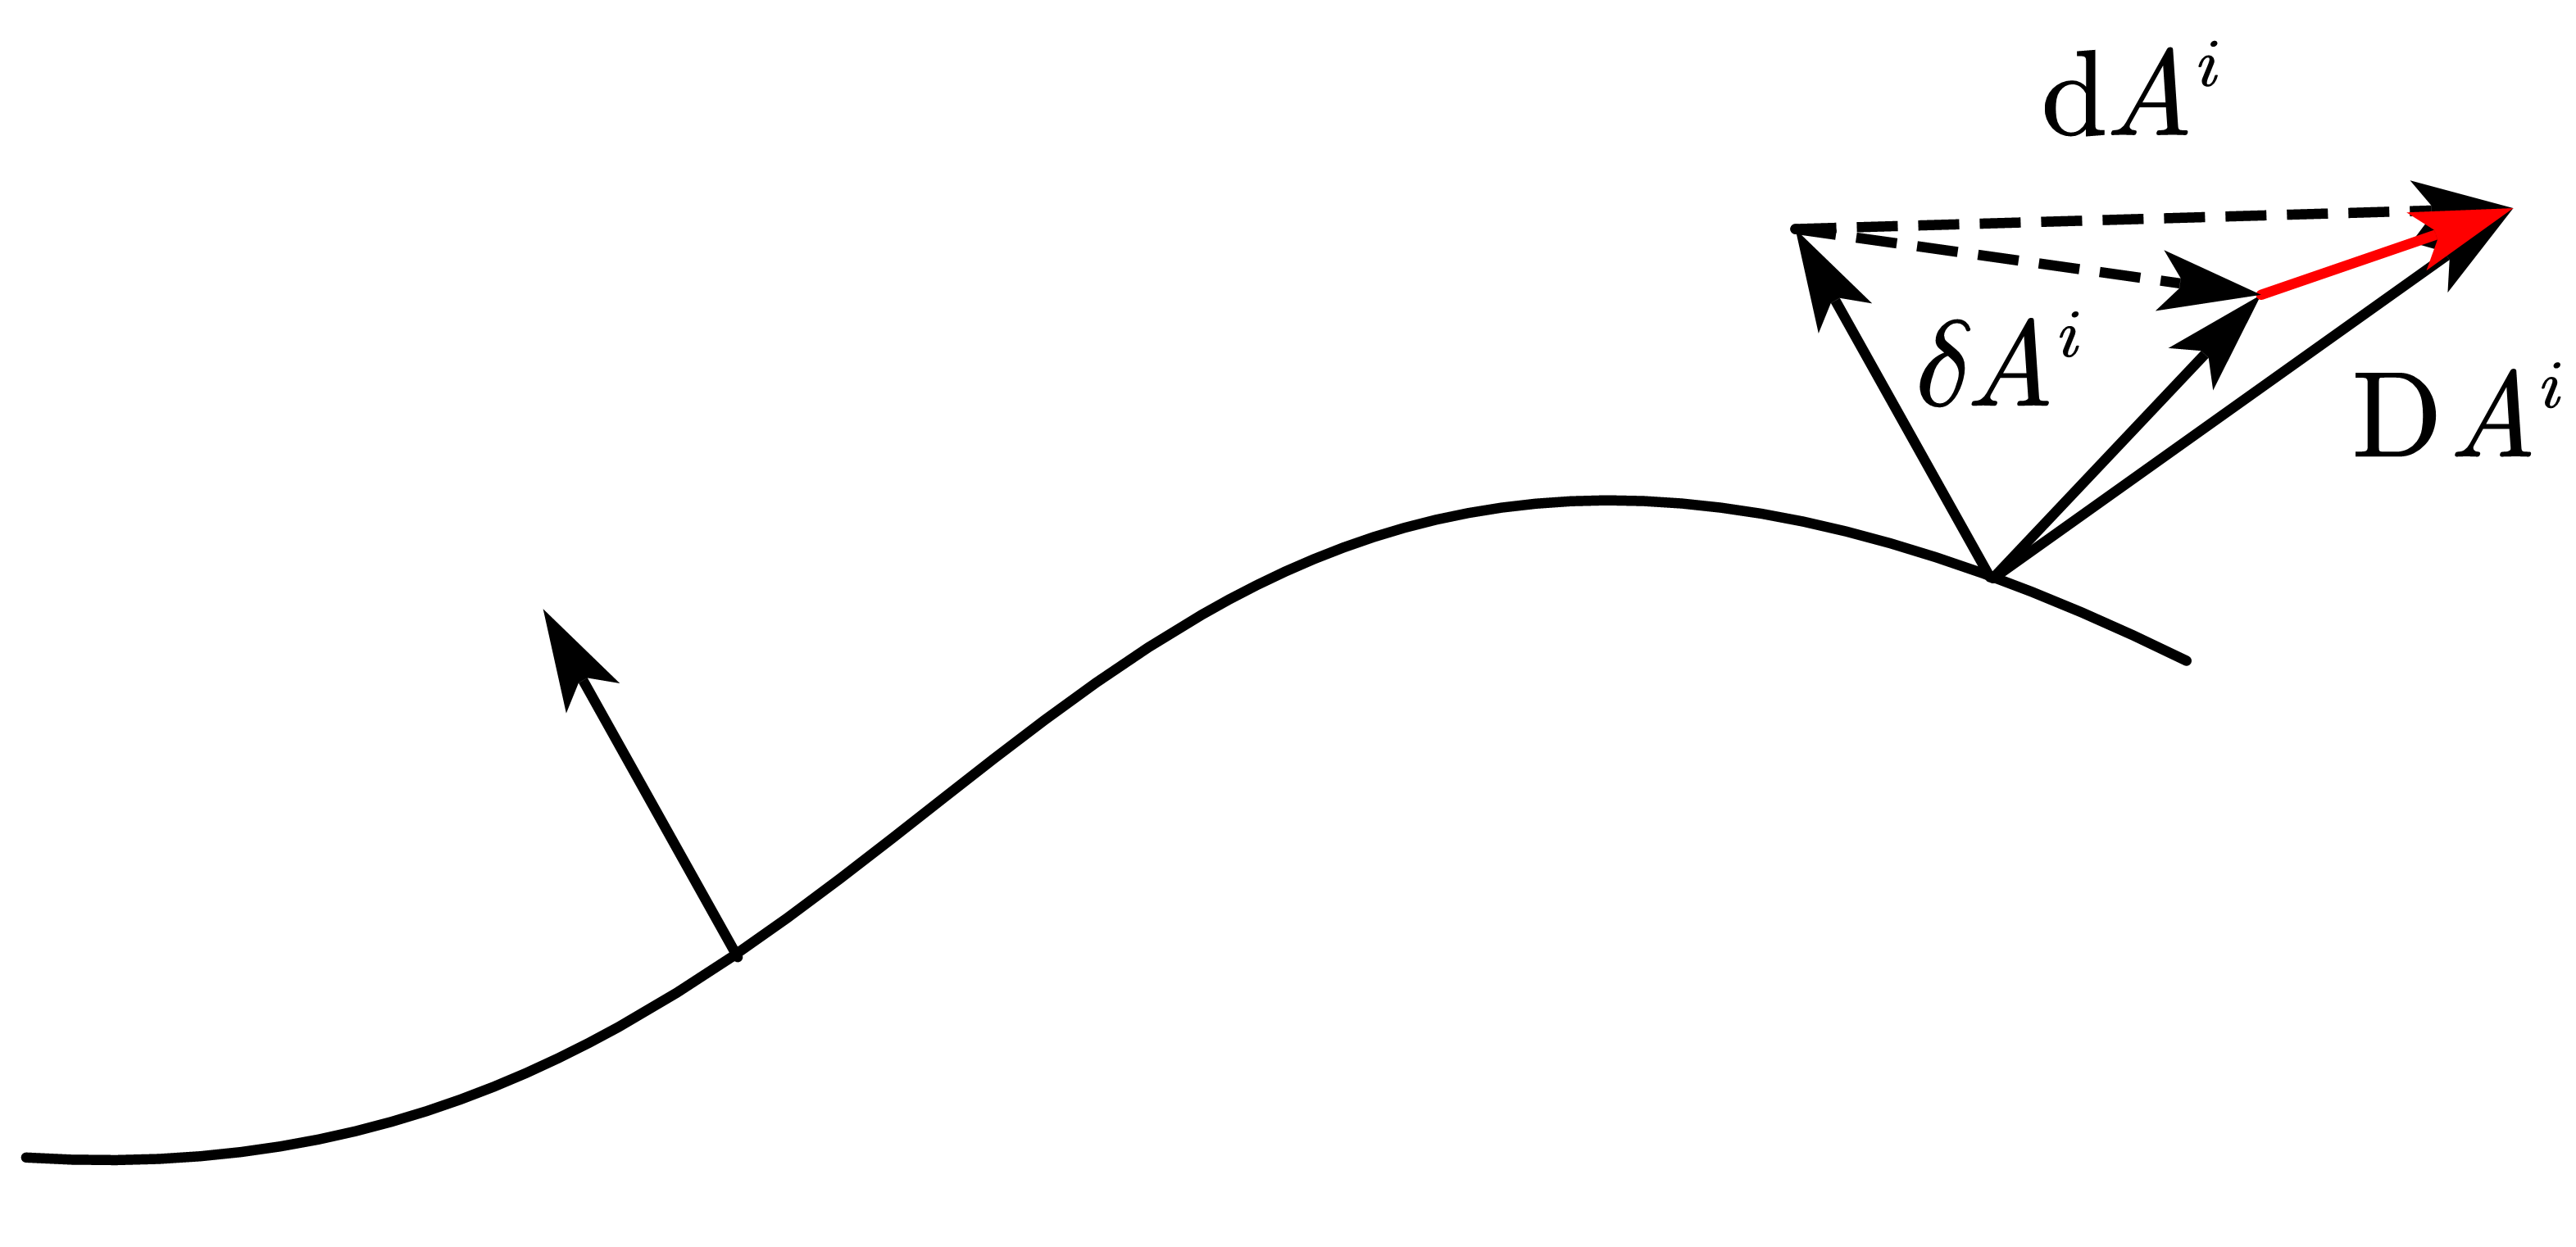
\includegraphics[width=8cm]{figure/CovariantDifferential.png}
\end{center}

我们希望计算微小坐标变化下引起的矢量的变动。如果直接把两个矢量相减,得到的是$\dif A^i$。但空间是弯曲的,假如把一个矢量沿着空间“平行移动”到与另一个矢量同起点,相对于之前的矢量,发生的变化是$\delta A^i$。协变微分就是图中的红线,即将一个矢量平行移动后计算的微分(如果两个矢量不是同起点,不能直接相减)。
\subsection{曲率}
\begin{empheq}[box=\fbox]{align}
R^i_{klm}&=\pdv{\Gamma^i_{km}}{x^l}-\pdv{\Gamma^i_{kl}}{x^m}+\Gamma^i_{nl}\Gamma_{km}^n-\Gamma_{nm}^i\Gamma_{kl}^n\mtag{黎曼曲率张量}\\
R_{iklm}&=g_{in}R^n_{klm}\\
R_{ik}&=g^{lm}R_{limk}=R^l_{ilk\cdot}\mtag{Ricci张量}\\
R&=g^{ik}R_{ik}=g^{il}g^{km}R_{iklm}\mtag{曲率标量}
\end{empheq}

\paragraph*{曲率张量的性质}以下前两个式子是说它关于$ik$和$lm$的第一对是反对称的。
\begin{empheq}{align}
R_{iklm}&=-R_{kilm}=-R_{ikml}\nonumber\\
R_{iklm}&=R_{lmik}\nonumber\\
R_{iklm}+R_{imkl}+R_{ilmk}&=0\nonumber\\
R^k_{ijl}+R^k_{jli}+R^k_{lij}&=0\mtag{第一比安基恒等式}\\
R^k_{ijl;h}+R^k_{ilh;j}+R^k_{ihj;l}&=0\mtag{第二比安基恒等式}
\end{empheq}
\section{空间坐标系}
\subsection{极坐标}\label{polar-coord}
\begin{center}
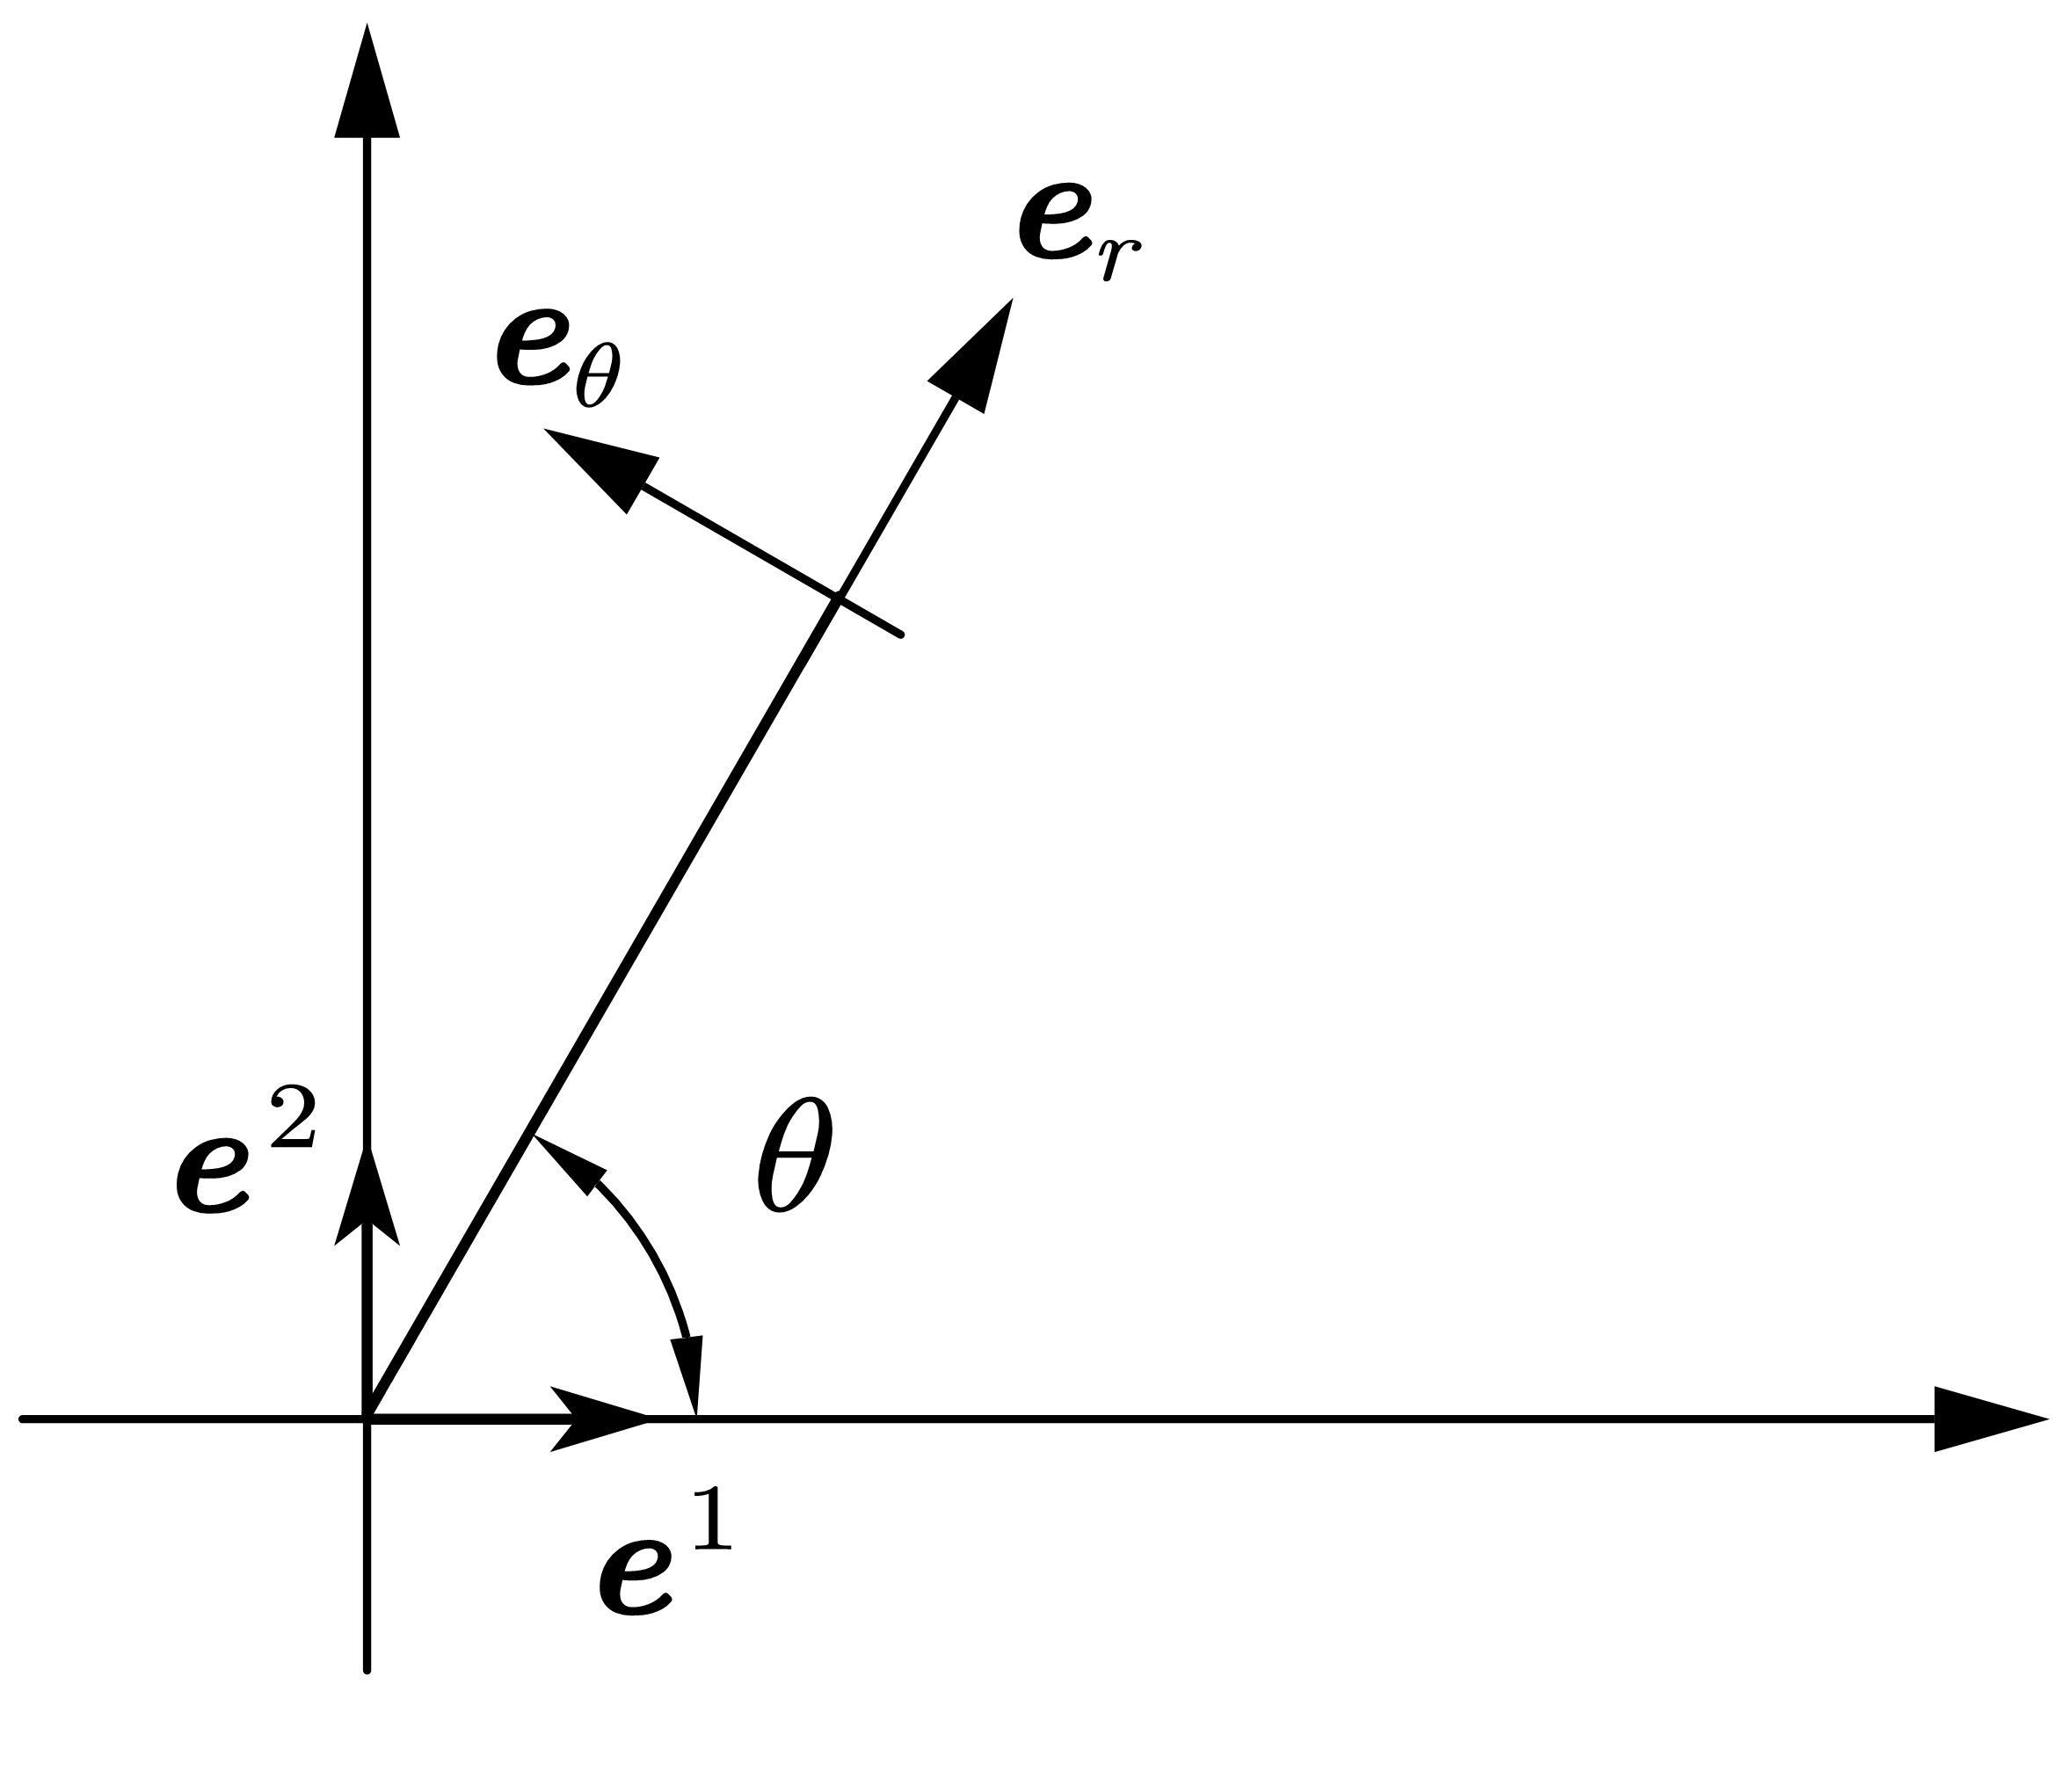
\includegraphics[width=5cm]{figure/polar-coord.png}
\end{center}

\begin{empheq}[left=\empheqlbrace]{align*}
x&=r\cos\theta\\
y&=r\sin\theta
\end{empheq}
求解
\[
(g_{ij})=\begin{bmatrix}
g_{rr} & g_{r\theta}\\
g_{\theta r}&g_{\theta\theta}
\end{bmatrix}=\begin{bmatrix}
1&0\\
0& r^2
\end{bmatrix}
,\quad (g^{ij})=(g_{ij})^{-1}\begin{bmatrix}
	1&0\\
	0& \frac{1}{r^2}
\end{bmatrix}\]
从度量中可以看出,极坐标系是正交坐标系。另外有基变换
\begin{empheq}{align*}
\bm{e}_r&=\pdv{x_i}{r}\bm{e}^i=\cos\theta\bm{e}^1+\sin\theta \bm{e}^2\\
\bm{e}_\theta&=\pdv{x_i}{\theta}\bm{e}^i=-r\sin\theta\bm{e}^1+r\cos\theta\bm{e}^2
\end{empheq}
\subsection{柱坐标}

\subsection{球坐标}
\subsubsection{坐标表示}
这里使用物理学中的约定。

\begin{center}
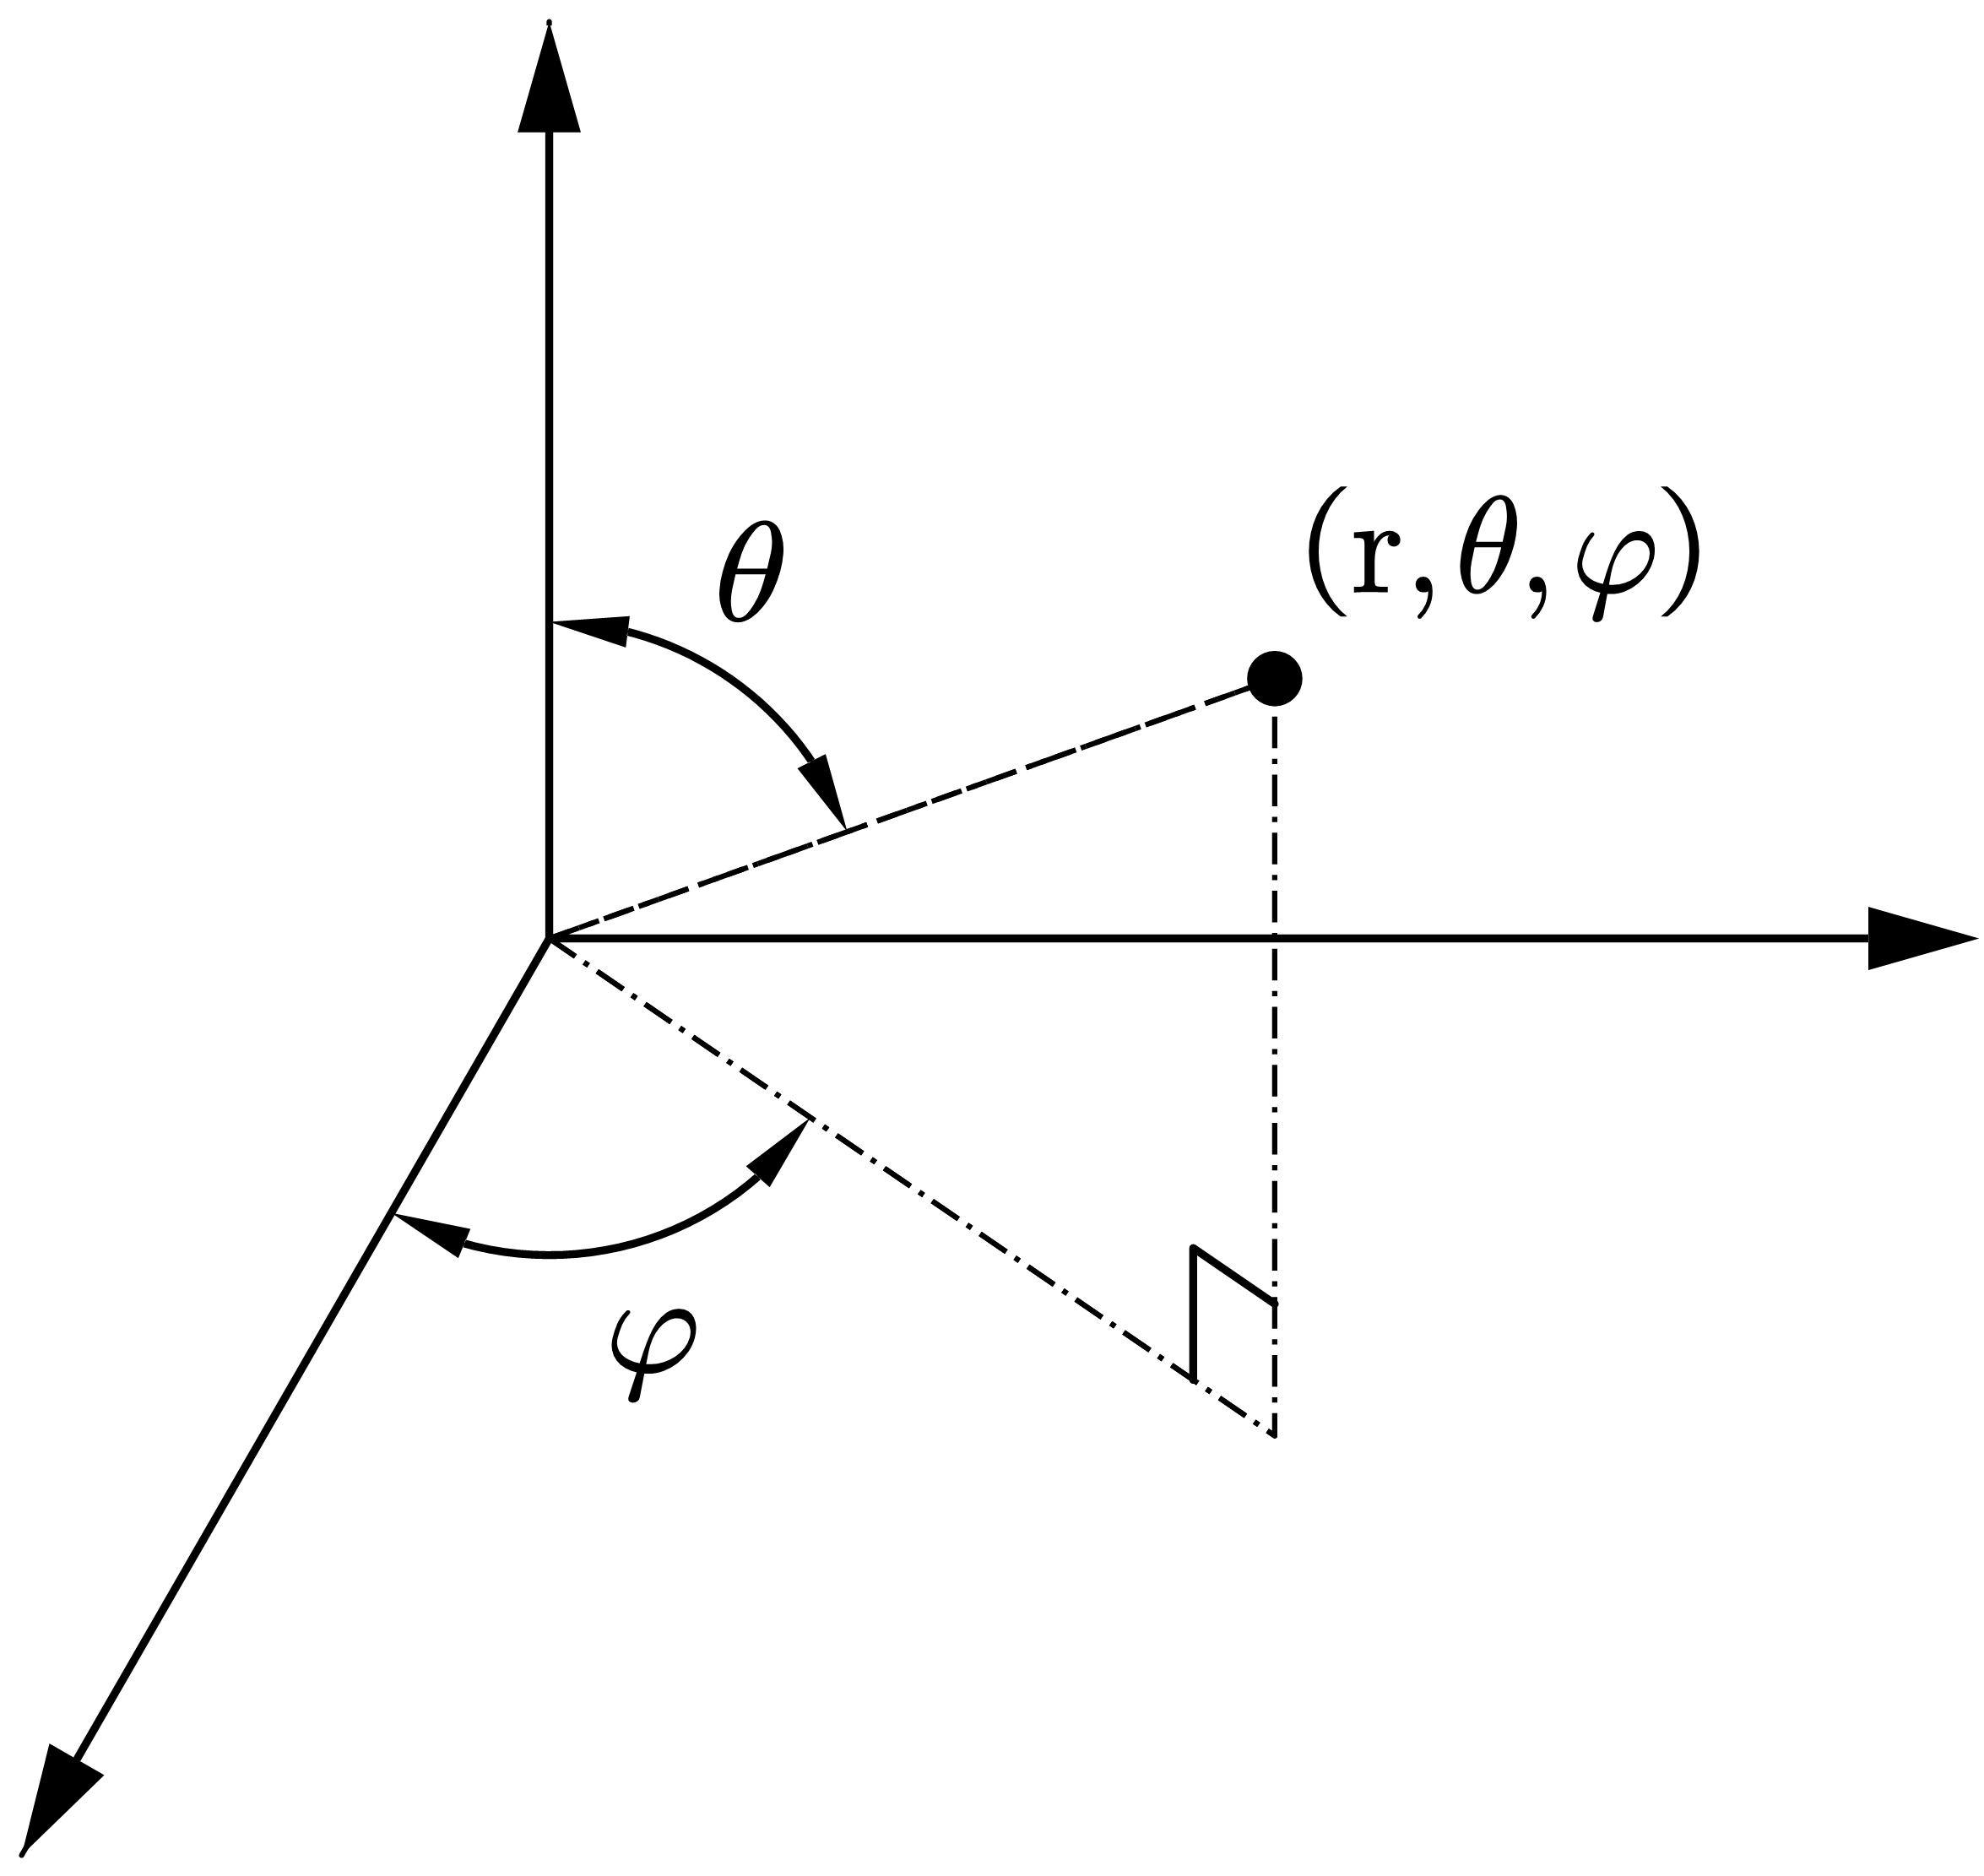
\includegraphics[width=4cm]{figure/Sphere3D.png}
\end{center}
\begin{empheq}[left=\empheqlbrace]{align}
x&=r\sin\theta\cos\phi\\
y&=r\sin\theta\sin\phi\\
z&=r\cos\theta
\end{empheq}

\subsubsection{微分公式}
\begin{center}
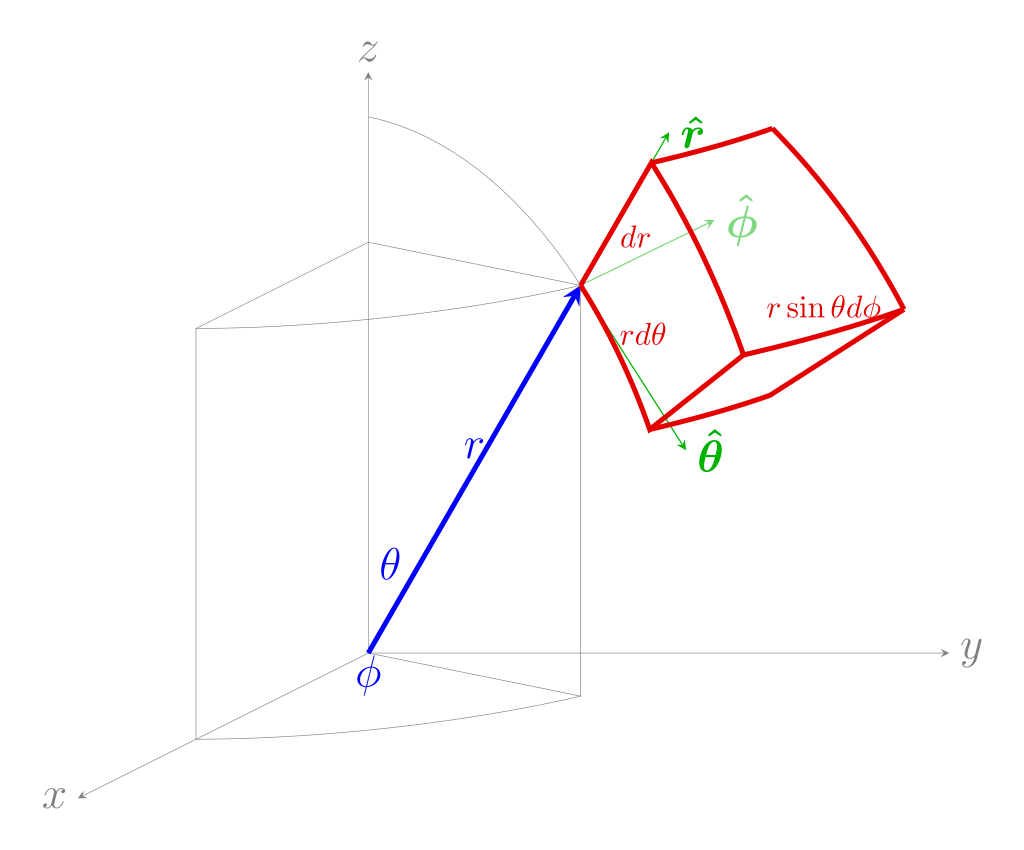
\includegraphics[width=6cm]{figure/Sphere3DDiff.png}
\end{center}

\begin{description}
\item[线元素] 从$(r,\theta,\varphi)$到$(r+\dif r,\theta+\dif \theta,\varphi+\dif \varphi)$的无穷小位移,表示为
$$\dif \bm{r}=\dif r \hat{\bm{r}}+r\dif\theta\hat{\bm{\theta}}+r\sin\theta\dif\varphi\hat{\bm{\varphi}}$$
$\hat{\bm{r}},\hat{\bm{\theta}},\hat{\bm{\varphi}}$为单位矢量。
\item[体积元素] $$\dif V=r^2\sin\theta\dif r\dif\theta\dif\varphi$$
\item[梯度公式] $$\nabla f=\frac{\partial f}{\partial r}\hat{\bm{r}}+\frac{1}{r}\frac{\partial f}{\partial \theta}\hat{\bm{\theta}}+\frac{1}{r\sin\theta}\frac{\partial f}{\partial \varphi}\hat{\bm{\varphi}}$$
\item[拉普拉斯算子] $$\nabla^2f=\frac{1}{r^2}\frac{\partial}{\partial r}\left(r^2\frac{\partial f}{\partial r}\right)+\frac{1}{r^2\sin\theta}\frac{\partial }{\partial\theta}\left(\sin\theta\frac{\partial f}{\partial \theta}\right)+\frac{1}{r^2\sin^2\theta}\frac{\partial^2f}{\partial \varphi^2}$$
\end{description}


\section{微分形式}
